\documentclass[pldi]{sigplanconf-pldi15}

\usepackage{url}                  % format URLs
\usepackage{listings}          % format code
\usepackage[colorlinks=true,allcolors=purple,breaklinks,draft=false]{hyperref}   % hyperlinks, including DOIs and URLs in bibliography
% known bug: http://tex.stackexchange.com/questions/1522/pdfendlink-ended-up-in-different-nesting-level-than-pdfstartlink
\newcommand{\doi}[1]{doi:~\href{http://dx.doi.org/#1}{\Hurl{#1}}}   % print a hyperlinked DOI
\usepackage{amssymb}
\usepackage{todonotes} %TODO Remove for final submission
\usepackage{minted}

\newcommand{\TODO}[1]{[\textsl{#1}]}
\newcommand{\code}[1]{\texttt{#1}}
\newcommand{\package}[1]{\code{#1}\cite{#1}}



\setcounter{tocdepth}{4} %TODO Remove for final submission

\begin{document}

\lstset{basicstyle=\footnotesize\ttfamily,mathescape=true,basewidth=0.5em}

\conferenceinfo{PLDI '15}{June 12---20, 2015, Portland, OR, USA.}
\copyrightyear{2015}
%\copyrightdata{}

%\titlebanner{banner above paper title}        % These are ignored unless
\preprintfooter{DRAFT - do not distribute}   % 'preprint' option specified.

\title{Efficient Multiple Dispatch in Julia}
%\subtitle{Subtitle Text, if any}

\authorinfo{Jeff Bezanson \and Jake Bolewski \and Jiahao Chen \and Stefan Karpinski \and Jean Yang \and Alan Edelman}
	{Massachusetts Institute of Technology}
	{bezanson@mit.edu, jake.bolewski@gmail.com, jiahao@mit.edu, stefan@karpinski.org, jeanyang@mit.edu, edelman@mit.edu}

\maketitle

\begin{abstract}
The goal of scientific programs is often to create experiments rather than to
build robust systems. Because scientific programs frequently involve operating
over reified data values with difficult-to-predict types, it is often easier
for scientific programmers to use dynamically typed languages. Unfortunately,
dynamic types often make it difficult to execute code efficiently. In this
paper, we describe the type system and multiple dispatch mechanism for the
Julia programming language, specialized for scientific computing. Julia has a
novel semantics based on efficient multiple dispatch. Julia combines
programmer-specified type tags with a type inference engine to statically
optimize method dispatch. Julia is dynamically typed in that the compiler does
not statically reject ill-typed programs, but Julia is designed to optimize
static type and dispatch inference. We describe the Julia language and type
system and our implementation of type inference and multiple dispatch
mechanisms for Julia. To demonstrate the relevance and potential impact of
designing a language based around multiple dispatch, we also describe the
manifestations of multiple dispatch in Julia's standard library.
\end{abstract}

\category{D.3.3}{PROGRAMMING LANGUAGES}{Language Constructs and Features}

\terms Languages, Multiple dispatch, Multimethods

%\keywords
%Language design, run-time system

\tableofcontents %TODO remove for final submission

\section{Dynamic languages are useful for technical computing}

\begin{quote}
	[L]a math\'ematique est l'art de donner le m\^eme nom \`a des choses
	diff\'erentes... Quand le langage a \'et\'e bien choisi, on est tout \'etonn\'e
	de voir que toutes les d\'emonstrations, faites pour un objet connu,
	s'appliqu\-ent imm\'ediatement \`a beaucoup d'objets nouveaux, on n'a rien \`a
	y changer, pas m\^eme les mots, puisque les noms sont devenus les
	m\^emes... c'est l'un des caract\`eres auxquels on reconna\^it les faits \`a
	grand rendement, ce sont ceux qui permettent ces heureuses
	innovations de langage. \cite{Poincare1908}
	
	\textit{Mathematics is the art of giving the same name to different
	things... When the language has been well chosen, one is amazed to see
	how all the demonstrations, made for a known object, apply immediately
	to many new objects, one has nothing to change, not even the words
	since the names have become the same... this is one of the
	characteristics by which one recognizes high-yield facts, they are the
	facts which permit successful innovations of language.}
\end{quote}

Engineers, mathematicians and scientists routinely write software for
computational simulations and data analysis to discover new insights.
Users writing code for the purposes of discovery often by definition do not
know what computations they need upfront, but rather discover what they want by
iterating through several different prototypes. Consequently, technical
computing code is often the product of an organic process of continuous
experimentation, rather than derived from formal software engineering
specifications.

Static languages focus on being able to prove correctness of programs, and
compilers usually contain features like type checkers which constrain the set
of allowed programs in favor of provable correctness. Code written in static
languages must be able to account for all possible behaviors of the algorithms
implemented for all possible input values. All these possible code paths must
stated at compile time, posing challenges for authors of technical codes which
often work on enormous inputs and may fail in subtle ways that require further
investigation and mitigation. Furthermore, these static analyses for
correctness tend to concern themselves with only the interface to data types,
not with their internal representation. Consequently, the formal logic of
program correctness does nothing for user concerns about performance, since
they abstract away memory layout details which is crucial for understanding the
impact of hardware factors such as bus latency and bandwidth. In contrast,
dynamic languages embody a realist philosophy: programs are not checked for
correctness, but are executed until termination or when a runtime error is
thrown. The focus is to make sense out of whatever program a user may write.
Thus dynamic languages are more permissive and expressive in ways that are more
naturally suited for rapid prototyping and experimentation.

In other words, a scientist will often run a program in order to find out what
it does---\emph{proving} anything about what it does would be premature, and an
unwelcome distraction. As a result, dynamic languages like MATLAB, Python and R
have become popular amongst technical computing users for writing prototype
codes. However, code written in these languages are difficult to execute
performantly; the dynamic nature of these languages pose significant challenges
for implementers to transform code into efficiently executable forms. Technical
computing users thus face a dilemma known as the two-language problem: it is
easier to prototype code in a dynamic language, but faster to run code written
in a static language. 

Julia is a dynamic language designed with the ambitious goal of eliminating the
false dichotomy between dynamism and speed~\cite{Bezanson2012,Bezanson2014b}.
The language features several different mechanisms for expressing polymorphism,
namely:

\begin{itemize}
	\item A user extensible type system featuring subtyping and parametric
		types, and
	\item A user extensible generic function system with dynamic multiple
		dispatch
\end{itemize}
%
which together naturally express the polymorphism inherent in technical
computing. Julia's implementation also features a just-in-time compiler which
performs extensive static optimizations such as:

\begin{itemize}
	\item Automatic type inference, which minimizes the overhead of dynamic
		multiple dispatch and largely eliminates the need for explicit
		type annotations in function bodies,

	\item Tuple elimination,
	\item Function inlining, and
	\item Other compiler optimizations such as dead code elimination that
		are provided by the LLVM library~\cite{Lattner2004}.
\end{itemize}

This paper aims to explain how Julia's language constructs and compiler
optimizations conspire to provide expressiveness without compromising
performance, by carefully designing a language that is purposely amenable to
static analysis. When combined with an extensive base library for parallel
execution and numerical analysis, Julia provides a convenient environment for
rapid prototyping of new analytics which can also be deployed performantly,
often within a factor of two of the speed of native, hand-written C code.



\section{Type system}

Julia is a dynamic language, i.e.\ it has no static semantics. As such, Julia
does not have types in the strict sense, but rather run-time type tags used to
differentiate heap-allocated objects~\cite[Section 11.10, p. 142]{Pierce2002}.
Nevertheless, the formal theory of dynamic type tags is well-defined as static
promises that are coerced at run-time into 
types~\cite{Henglein1994,Shields1998,Baars2002}, and there should be no ambiguity
in using the terms ``type'' and ``type tag'' in this paper. This
section aims to describe how dynamic type tags can be used, not for type
checking to statically reject ill-typed programs, but rather to disambiguate
objects and facilitate dispatch in ways similar to static
types~\cite{Tratt2009,Kell2014}.

All values in a dynamically typed language have two semantic components:
a \emph{tag} and some \emph{data}. The tag classifies the data, which are the
contents of some block of memory whose format is set by the programming
language. Tags are useful for both users and compilers for deciding what to do
to values, but incur overhead which increases the memory footprint of a data
item. This overhead motivates most dynamically typed languages to simplify and
minimize their tag systems.

In contrast, Julia's types are designed for expressiveness, resulting in fewer
components to the language design. An important example is arrays, which are
special cased in some languages for performance reasons, but in Julia are
described as a particular kind of parametric type, with the type parameter
encoding information about memory layout.~\cite{Bezanson2014}. In general,
Julia's types allowing programs to reason about:

\begin{itemize}
\item when code is applicable (dispatch),
\item what to specialize on,
\item memory layout, and
\item what can be statically known about a potential value.
\end{itemize}
%
Furthermore, types are first-class values, allowing programs that can compute
on types and reason about all of the above.

\TODO{Orphans}
\begin{quote}
	[I]t behooves the language designer to incorporate distinctions between
	types into his language. Doing so permits an implementer of the
	language to choose different representations for different types of
	objects, taking advantage of the limited contexts in which they will be
	used.
\end{quote}

Statically determining all tags is generally not possible.

Parametric polymorphism like template specialization but dynamic.

the core of functional programming languages, like those in the ML family, support both parametric polymorphism and record subtyping, which can be expressed in System F<:.

Static languages like Haskell have typeclasses\cite{typeclass}, but you'll need
to anticipate all the necessary use cases ahead of time because everything is
resolved statically and also know all the cases you'll be in at compile time.
Dynamic languages provide only dynamic bindings, which means that programmers
don't have to reason about the differences between static and dynamic
semantics, and dynamic binding is more general anyway.

A key design of the Julia type system is that in enables polymorphism by having type parameters and subtyping relations.

The challenge in designing such a type system are in specifying how
tags can be computed and how the subtyping relationships work.

Type promotions are written as user-level code to compute new types.

\paragraph{Types are values: Fewer language constructs for user simplicity}
Being able to write things like \code{Array} as a synonym
for \code{Array\{T\}}.  Such synonyms are valuable for composability when
writing methods that are agnostic about the type parameter \code{T}.  Methods
that cared about \code{T} can be defined with a type signature that explicitly
mentions \code{T} and methods that did not care about \code{T} can have a type
signature that left it out.  The ability to leave out type parameters in
function signatures contrasts with other languages \TODO{like which} which
require explicit specification of all type parameters, resulting in users
having to write redundant code blocks whose sole purpose is handle the nuisance
parameter.


\subsection{Kinds of types}

Julia has different kinds of types which can be formally summarized as:

\begin{lstlisting}
Type ::= Abstract | Data | Tuple | ForAll | Union | Singleton
Abstract ::= Name (P) Super }
Data ::= Name (P) Super Repr } invariant, nominative
Tuple ::= (T1, T2, ...) | (T1, T2, ..., Tn, ...) } covariant
ForAll ::= $\forall$ (lb <: T <: ub) . Type
Union ::= U (T1, T2, ...)
Singleton ::= Lift Value
TypeVar ::= lb <: Name <: ub

Tag ::= Data | Tuple
\end{lstlisting}

\begin{description}

\item[Data constructor/Tag types] are types with associated constructors. They
	are further subdivided into:
	\begin{description}
	
	\item[Bits types] like double precision floating point numbers
	(\verb|Float64|) and 32-bit signed integers (\verb|Int32|), which can
	be stored unboxed as raw bits without tag overhead,

	\item[Abstract data types] which have an internal representation
		declared with the \verb|type| keyword, and
		
	\item[Immutable types] which are similar to abstract data types
		declared with the \verb|immutable| keyword, but whose internal
		variables are immutable, thus potentially allowing for unboxed
		representations.

	\end{description}


\item[Tuple types] \code{(T1, T2,...)} which are constructed from the Cartesian
	product of zero or more existing types \code{T1}, \code{T2},
	etc.~\cite[Sec. 11.7]{Pierce2002} Tuples are covariant.

\item[Abstract types] define an uninstantiable type with no declared
	representation. They are used as declared supertypes of leaf types
	(which are concrete and instantiable).

\item[Singleton types] are constructed with the \code{::Type\{T\}} syntax and
	are used for primarily for computations on types themselves, such as
	type promotions, and for dispatch. \TODO{Sorting algorithms example: used
	more for dispatch as shorthand for type with no parameters.}

\item[Union types] declared as \code{Union(T1, T2,...)} are the join of zero,
	or two or more, types \code{T1}, \code{T2}, ...~\cite[Sec.
	15.7]{Pierce2002}
	%
	\begin{equation}
		\texttt{Union}(T_1, T_2, ..., T_N) = \bigwedge_{i=1}^N T_i 
	\end{equation}
	%
	The union with zero types, \code{Union()}, is simply the bottom type.
	%
	Julia's \code{Union}s are untagged and disjoint, which allows for some
	simplifications in their construction:
	\begin{itemize}
		\item If there are types \code{S} and \code{T} obeying the
			subtyping relation \code{S <: T} in the union
			constructor, then \code{S} is deleted ($\beta$-reduced)
			from the final union type constructed. This
			simplification includes the special case where \code{S}
			and \code T are identical.

		\item A union type \code{Union(T)} with a single type parameter
			\code{T} is identical (by $\eta$-reduction) to just
			\code{T}.
	\end{itemize}

\item[\code{TypeVar}s] are not types, but are quantifications over sets of
	types. They are used to define constraints on type parameters in type
	constructors, and also
	
\item[\code{ForAll} types] which quantify over all types between a lower bound
	and upper bound.

\end{description}

Julia's type system supports two mechanisms for polymorphism, namely subtyping
and type parameters. 


\subsection{Subtyping}

Julia supports strong behavioral subtyping: objects of a given type can be
replaced with objects of their subtype without altering desirable program
behavior. This property is called the Liskov substitution
principle~\cite{Liskov1974}.

Julia requires allows user-defined types to have exactly one declared supertype.
If no supertype is declared explicitly, the supertype is assumed to be \code{Any}.

\subsection{Type parameters}

Parametric types are invariant.
The conventional wisdom is that type safety requires covariance if components
are read but not written, and contravariance if they are written but not
read~\cite{Castagna1995}. As type parameters can represent the types of mutable
fields in a \verb|type| which can be read or written, then the only safe choice
is invariance.

\paragraph{Example of user-definable type}

Example: the \code{Complex} type defined by

\begin{minted}{julia}
immutable Complex{T<:Real} <: Number
    re :: T
    im :: T
end
\end{minted}

has two declared fields, \code{re} and \code{im}. Each of these fields has the
type annotation \code{::T}. The type parameter \code{T} is constrained to be a
subtype of \code{Real}, and \code{Complex} itself has a declared supertype
which is \code{Number}.

\code{Complex} comes with a default, implicitly defined inner constructor

\mint{julia}|Complex{T<:Number}(re::T, y::T) = new(re, im)|
%
which makes use of a special intrinsic function \code{new} to allocate new
memory for the fields \code{re} and \code{im}. Inner constructors can be
defined by the user, in which case the default inner constructor is not
generated.

An instance of \code{Complex} can be created using the inner constructor, e.g.\

\mint{julia}|z = Complex{Float64}(0.0, 1.0)|

whose fields can be accessed directly as \code{P.x} and \code{P.y} respectively~
\footnote{\code{P.x} is desugared into the equivalent Julia code \code{getfield(P, x)}.
\code{getfield} is Julia's field accessor function.}

\TODO{Talk about the psychological implications of types.}

Is there multiple inheritance?
No, but it's been discussed (https://github.com/JuliaLang/julia/issues/5)


\paragraph{Subtyping relations and the type lattice}

The existence of the subtyping relation \verb|<:| imbues Julia types with
lattice structure~\cite{Scott1976}, with a meet operator $\wedge$ computing the
type intersection (\verb|typeintersect|), and a join operator \TODO{pin
symbol?} which creates union types. Furthermore, the lattice is complete, as it
is live on a complete lattice bounded below by the bottom type $\bot$ or
\verb|Union()|, and bounded above by the top type $\top$ or \verb|Any|. As we
shall see later, the existence of type lattice allows for sophisticated type
inference algorithms to be used.  

In practice, joins are easy to construct by forming unions.  Meets are more
difficult as Julia does not natively support intersection types.

\paragraph{Subtyping is not set embedding!}
Another aspect of the type system that can be confusing to new users is that
subtyping can express some, but not all, mathematical embeddings between sets
of allowed values.

Examples:

- Each 8-bit unsigned integer (Uint8) represents an integer in the set {0, 1,
\dots, 255}. Each of these in turn has an exact representation as a
double-precision floating point number (Float64). Nevertheless, Uint8 is not a
subtype of Float64.

- Int64 <: Real: each 64-bit signed integer (Int64) is a real number.

- Each value of \verb|Complex{Int64}| is a Gaussian integer, i.e. a complex number
where each component is an integer, and so each \verb|Complex{Int64}| is in 1:1
correspondence with a value in \verb|Complex{Integer}| and also in \verb|Complex{Real}|.
Nevertheless, \verb|Complex{Int64}| is a subtype of neither \verb|Complex{Integer}| not
\verb|Complex{Real}| due to parametric invariance. However, all of these are subtypes
of Complex.

- Real is not a subtype of Complex because for each type T that is a subtype of
Real, there is a corresponding instantiable type Complex{T}. None of these
correspond to Real since there is no T such that Complex{T} is a one-component
number, and each concrete type only has $\bot$ as its subtype.  


\paragraph{\code{typeof}}

You can define \code{typeof} axiomatically as having the following behavior on a \code{value=(bits, tag)} pair:

\begin{minted}[frame=lines,framesep=2mm]{julia}
typeof(bits, tag) = (tag, DataType) #Returns a value
\end{minted}

\code{typeof} has a fixed point, namely \code{(DataType, DataType)}. This is
also true in other dynamic languages, e.g.\ Python (CPython). In other
languages like Haskell, \code{typeof(DataType) = Kind}, etc. Static languages
can just truncate the tower of metatypes and also refuse to type-check code
that reasons about types and kinds too far up the hierarchy. In fact, early
versions of Haskell did not allow for programs to reason about kinds at the
data type level due to the lack of kind polymorphism~\cite{haskellkindtypes}.

\TODO{There is a subtlety about typeof's behavior. typeof is a projection;
typeof(not-a-type) produces a DataType, which projects non-type values onto
types. It also has the effect of lifting non-type values onto a type lattice;
the latter is defined only for values that are DataTypes.}

\TODO{The main novelty and challenge is explaining type parameters and
typevars. Currently typevars are not first-class objects in Julia; you can't
pass them to a function. Expressions of the form \code{T<:SomeType} don't have
an independent existence outside a function signature that also contains the
\code{\{T...\}} construction.}

\subsection{Type promotion}

\subsection{Example: modular integer arithmetic with \code{lcm}}

Here's an example of a type parameter computed with the \code{lcm} function:

\begin{minted}[frame=lines,fontsize=\footnotesize,
               framesep=2mm]{julia}
import Base: convert, promote_rule, show, showcompact

immutable ModInt{n} <: Integer
    k::Int
    ModInt(k) = new(mod(k,n))
end

-{n}(a::ModInt{n}) = ModInt{n}(-a.k)
+{n}(a::ModInt{n}, b::ModInt{n}) = ModInt{n}(a.k+b.k)
-{n}(a::ModInt{n}, b::ModInt{n}) = ModInt{n}(a.k-b.k)
*{n}(a::ModInt{n}, b::ModInt{n}) = ModInt{n}(a.k*b.k)

convert{n}(::Type{ModInt{n}}, k::Int) = ModInt{n}(k)
convert{n}(::Type{ModInt{n}}, k::ModInt) = ModInt{n}(k.k)
promote_rule{n}(::Type{ModInt{n}}, ::Type{Int}) = ModInt{n}
promote_rule{m,n}(::Type{ModInt{m}}, ::Type{ModInt{n}}) =
    ModInt{lcm(m,n)}

show{n}(io::IO, k::ModInt{n}) = print(io, "$(k.k) mod $n")
showcompact(io::IO, k::ModInt) = print(io, k.k)

julia> a = ModInt{12}(18278176231)
7 mod 12

julia> b = ModInt{15}(2837628736423)
13 mod 15

julia> a + b
20 mod 60
\end{minted}

The type of the result \code{a + b} depends on the types of \code{a} and \code{b} via \code{lcm}.



\section{Generic functions and multimethods}

As \cite{Poincare1908} noted in the opening quote, mathematical thought is
naturally polymorphic.  Multimethods are a natural mechanism for capturing such
polymorphism.  Consider an operation as fundamental as multiplication: an
expression like \verb|a*b| can mean:

\begin{itemize}
	\item a matrix--matrix product,
	\item a matrix--vector product, or
	\item a scalar--vector product,
\end{itemize}
%
to name just a few possibilities. A generic function system supporting
multimethods allows for the \verb|*| function to be polymorphic, expressing a
common metaphor for different kinds of multiplication which can be
disambiguated by the types of \verb|a| and \verb|b|. In contrast, languages
supporting only classes cannot capture the full extent of polymorphism in
\verb|*| in method dispatch: as classes inherently support only single dispatch
on the first argument, each method \verb|*| defined for each class \verb|a|
must contain different code blocks for each possible type of \verb|b|, thus in
practice requiring multiple dispatch to be emulated using virtual methods and
visitor patterns~\cite{designpatterns}. Furthermore, implementing binary methods can
require knowing the internal representation of both objects \verb|a| and
\verb|b|, especially for performance reasons~\cite{Bruce1995}. Such knowledge
fundamentally corrupts the abstraction of class-based encapsulation, as the
methods associated with \verb|a| must know implementation details of all
possible objects \verb|b| that \verb|a| may interact with, thus further
compounding the problem of enumerating all possible code paths at compile time.
In contrast, there is no abstraction leak associated with allowing a generic
function \verb|*| knowledge about the internal representations of the types it
works on.

Julia's generic function system can be extended with user-defined methods, thus
allowing for users to define new generic functions and extend existing
functions with new methods, or even overwrite existing methods to suit their
needs. Thus multiplications represented by \verb|*| can be extended, for
example, to multiplication between quaternions, or even to $N$-ary
matrix-matrix products, where associativity\footnote{Neglecting the lack of
exact associativity in some fields such as floating-point numbers.} allows
matrix-matrix products to be regrouped so as to minimize the total memory
footprint and operation count~\cite{Hu1984}.

\paragraph{Multiple dispatch allows dispatch on new types and new functions at the same time}
The needs of technical computing can exceed the abilities of most dispatch
systems.  In particular, it is usually not possible to have new behaviors that
intermix new types and new functions.  One group of languages allows you to
have new types but their dispatch upon existing functions cannot be defined.
Subtyping is the usual paradigm here, but it is closed because it assumes
you've covered all the cases explicitly.  Object oriented programming can be
seen as a solution around this problem, but in pure OO, objects have only
identity and have no interface protocol.  Classes are a mechanism for
implementing message sends, defining actions \textit{upon} an object.  The
other group of languages allows you to have new functions but not for existing
types.  Haskell typeclasses~\cite{typeclass} are a fixed collection of
interfaces; while additional functions can be defined, only the functions that
form part of the existing interface can interact with an existing type.

\TODO{Orphans/to flesh out}
The prices we pay for such flexibility:
- No encapsulation guarantees.  programs may at any point be able to peer into
the internal representation of types. As a result, type safety requires
stringent criteria on the allowed variances of types.
- Increased overhead of dynamic lookups for function dispatch: unlike in a single dispatch language, multiple lookups in method tables may be necessary to determine which method is most appropriate for dispatch~\cite{Bruce1995}.

\TODO{Is method table caching algorithm related to existing literature?}

\paragraph{Method sorting and dispatch mechanism}
\TODO{Describe}
Method tables are a sorted list of these types.
Implemented as \code{jl\_methtable\_t}

\subsection{Diagonal dispatch}

Diagonal dispatch is a special refinement of method dispatch that occurs when a
type parameter appears in more than position in the method signature, e.g.:

\verb|f{T}(x::T, y::T)|
%
Diagonal dispatch occurs only for concrete types \verb|T|. For example,
\verb|f(1, 2)| works as the arguments are of type \verb|(Int, Int)|, but not
\verb|f(1, 2.0)| as the arguments are of type \verb|(Int, Float64)|, even
though that tuple type is a subtype of \verb|(T, T)| where
\verb|T = Union(Int,| \verb|Float64)| or any larger union of \verb|Int| and
\verb|Float64|. Thus for diagonal dispatch to match only concrete \verb|T|s,
the tuple of arguments is treated \textit{not} covariantly, but rather,
\textit{invariantly}. Although this is an unusual special--casing of tuple
behavior, the greater specificity allowed by invariance makes diagonal dispatch
more useful in practice by matching only concrete types, particularly when
\verb|T| appears multiple times in the method signature, e.g.\ 
\verb|f{T}(x::T, y::T, z::T)| or even \verb|f{T}(xs::T...)|. 

The \textit{diagonal} nature of diagonal dispatch is apparent when considering
the dispatch table for the method \verb|f{T}| \verb|(x::T, y::T)|: when written
out as a table with all possible types of \texttt{x} and \texttt{y} along the
rows and columns as shown in Table~\ref{tab:diagonal}, the method dispatches
only along the diagonal of the table.

\begin{table}
\begin{tabular}{c | c c c c c}
	& \verb|Int| & \verb|Float64| & \verb|Bool| & \verb|Real| & $\cdots$ \\ \hline
	\verb|Int|     & \checkmark &  &  &  & \\
	\verb|Float64| &  & \checkmark &  &  & \\
	\verb|Bool|    &  &  & \checkmark &  & \\
	\verb|Real|    &  &  &  &  & \\
	$\vdots$       &  &  &  &  &
\end{tabular}
\caption{Dispatch table for the function \texttt{f} with method
\texttt{f\{T\}(x::T, y::T)}, showing that dispatch occurs only along the
diagonal with all possible types of \texttt{x} and \texttt{y} along the rows
and columns.}
\label{tab:diagonal}
\end{table}


\section{Type inference}

One key insight into the design of Julia is that static analysis can eliminate
the overhead of dynamic dispatch in many cases, thus allowing Julia code to run
at speeds comparable to analogous code written in fully compiled static
languages. The key static analysis technique is type inference, which can be
thought of as a process of describing data automatically: programs can accept
an \emph{arbitrary} value, discover its structure, and operate on it by
examining its tag.

\paragraph{Type inference is a key part of the language}
A somewhat unusual feature of julia is that we consider dataflow type inference a
key part of the language. Strictly speaking, this is an optional, external program
analysis that might be used for various purposes, chief among them implementing
an optimizing compiler. However, it is highly important to programmers since it
largely defines not the semantics, but the performance model of the language.

\paragraph{Dataflow captures intuition of control flow}
We feel that dataflow analysis, especially of forward flow, captures a piece of
the human intuition of how programs work: values start at the top and move through
the program step by step. For example, compilers are much more user-friendly
when they elide a possibly-uninitialized variable warning in

\begin{minted}[frame=lines,framesep=2mm]{julia}
int a;
if (cond)
    a = 1;
else
    a = 2;
f(a);
\end{minted}

The programmer knows that \code{a} is always initialized before use.

\TODO{Orphan}
automatic type inference allows many
explicit type annotations to be eliminated, thus resulting in shorter and more
reusable code.

\paragraph{Code transformations in the Julia compiler}
The Julia code is parsed, then macro expanded, then lowered into SSA form, then
type inference runs on the lowered code where the code paths are essentially
linearized with jumps. This form is relatively straightforward to map onto LLVM
IR and is also simpler to run dataflow analysis on. After type inference comes
tuple elimination, inlining and then conversion to LLVM IR where further
optimizations passes occur.

Type inference avoids explicit annotations and yet recovers almost enough information for performant dispatch. The goal is to dispatch onto machine types where possible and yet be flexible enough to support general code. Multiple dispatch was one part of the puzzle. The other part is type inference.

Type inference must be flow sensitive for a dynamic language since the type of a variable can change over the course of a program. Therefore we can't do Hindley Milner because it is flow insensitive. Instead, have to use dataflow-style static analysis for type inference.

Standard dataflow analysis makes use of the lattice structure of types to perform minimal fixed point analysis.

In general, type inference is NOT decidable! The set of pure terms which are typable in the λII-calculus in a given context is not recursive. So there is no general type inference algorithm for the programming language Elf and, in some cases, some type information has to be mentioned by the programmer. 

\paragraph{Dataflow analysis}
 flow-sensitive analysis, the topic of Section 4.5,
may improve precision in this case by allowing slots to have different types at different points in the target program.
More specifically, flow-sensitive analysis tracks the flow of control from assignments to reads of slots, attempting to
eliminate certain object types from the types of slots when control-flow properties make it impossible for them to
reach specific reads.

Need flow senstitive analysis because variable identifiers are allowed to be rebound and retyped at any point in the code. This rules out flow-insensitive type inference algorithms such as Hindley-Milner, which are popular in the ML family of languages.

What is the goal of the dataflow analysis? Primarily for static type inference. Eliminate runtime checks. Lattice-based. Kaplan-Ullman.
Problem is finding the tightest possible set of allowable types.
There are tweaks to the standard algorithm. One big thing is that dataflow analysis only goes in forward direction.
Kaplan-Ullman also doesn't treat parametric types
Julia also has a widening step.
Relies on types having only one supertype.

\TODO{What are the challenges?}

\TODO{What is the complexity?}

\TODO{What is the best way to express this?}

\TODO{bit of background}

\paragraph{Abstract interpretation and flow functions}
The basic idea is abstract interpretation with flow functions (in Julia, called
t-functions) to represent the types of variables going in and out of each basic
block.  Abstract interpretation is essentially about systematic reasoning about
approximations. For type inference the approximation we make is to figure out
what types come in and out of program fragments. Further approximation is
widening which provides looser bounds on the inferred types. 

In general it suffices to consider lattices which have only finite chains. The
point of view of DFA based on abstract interpretation [CC77, AH87]is to replace
the standard semantics of programs by an abstract semantics describing how the
instructions operate on the abstract values A. Formally,we assume a
monotone semantic functional $![.!] : Instr \rightarrow (A \rightarrow A)$
which assigns a function on A to each instruction.

\paragraph{Mohnen's algorithm}
We use Mohnen's algorithm which avoids explicit initialization of graphical
representations of code structures, but instead work on the static single
assignment (SSA) form of the lowered code and has program counters. SSA is easy
to use because def-use chains tend to be very sparse (very few flow edges) and
there is exactly one definition reaching use of each variable, which reduces
the time needed to analyze. Mohnen's algorithm uses less memory and has better
data locality than standard graphical constructions like Tenenbaum? Muchnick?
etc, and furthermore avoids explicit transformations between lowered code, SA
graphs and BB graphs. Whereas Mohnen demonstrates its use on constant
propagation, we nevertheless use it for forward type inference, where the
computation at a node is influenced by information from previous nodes in the
control flow.

\paragraph{Existence and termination}
Monotonic flow functions (a.k.a.\ transfer functions or t-functions) are essential.
Monotonicity implies flow functions preserve the ordering of approximations.
parametric invariance makes it easy to construct monotonic flow functions since invariance means disjoint lattice structure
complete lattice with top implies that we have descending chains, so meets exists so a lub exists done.
It is also crucial for dataflow algorithms to converge to a fixed point
The finite height assumption of a lattice is essential to prove termination.

\paragraph{Widening for convergence acceleration}
We also use widening as a convergence acceleration technique. Although widening
does not guarantee converging to a minimal fixed point, the analysis
nonetheless converges and that is good enough.  Widening also deals with
infinite types because there are heuristic cutoffs for the traversal into the
substructure of data types.



\section{Applications in technical computing}

\TODO{A good motivating example for types is $2^{64}$}

\subsection{Numerical linear algebra library}

Designing a general-purpose linear algebra library involves several different
layers of complexity, and has been described as implementing the following
meta-program~\cite{Demmel2007}:

{\small
\begin{verbatim}
(1) for all linear algebra problems
    (linear systems, eigenproblems, ...)
(2)  for all matrix types
     (general, symmetric, banded, ...)
(3)   for all data types (real, complex,
      single, double, higher precision)
(4)    for all machine architectures and
       communication topologies
(5)     for all programming interfaces
(6)      provide the best algorithm(s) available
         in terms of performance and accuracy
         (``algorithms'' is plural because
         sometimes no single one is always best)
\end{verbatim}
}
%
The six-tiered hierarchy neatly delineates how the basic collection of linear
algebra problems (1) have to be specialized by data representation (2-3) and
machine details (4), which are then used to decide which specific algorithms
(5-6) to use.

Many systems provide optimized implementations of standard libraries for
numerical linear algebra like BLAS (Basic Linear Algebra Subprograms) and
LAPACK (Linear Algebra PACKage). Computational routines can be customized
for individual microarchitectures and can reach a significant fraction of
theoretical peak FLOPS. However, these libraries inherit archaic Fortran 77
interfaces and hence tend to restrict routine names to six letters or shorter.
When combined with the lack of polymorphism in Fortran, the names are terse and
cryptic to nonexperts: a typical routine like \verb|DSTEV| solves the
eigenvalue problem (\verb|EV|) for symmetric tridiagonal matrices (\verb|ST|)
with double precision floating point entries (\verb|D|), and furthermore takes
eight positional arguments specifying the inputs, outputs, computation mode,
and scratch variables. The lack of polymorphism results in redundancy due to
lack of code reuse, which hinders the implementation of new algorithms (which
have to be reimplemented for each level of floating-point precision) and new
routines for such as mixed-precision and quad precision routines (which must
implement all the existing algorithms).

The code redundancy problem is largely ameliorated with the combination of type
polymorphism and dynamic multiple dispatch. The six-tiered hierarchy above maps
naturally onto different language constructs in Julia as follows:

\vspace{12pt}
\begin{tabular}{c l l}
	\hline
	Tier & Description & Language construct \\ \hline
	1 & linear algebra problems & generic function \\
	2 & matrix types & parametric types \\
	3 & data types & type parameter \\
	4 & machine architectures & method body \\
	5 & programming interfaces & generic function \\
	6 & (poly)algorithms & method body \\ \hline
\end{tabular}
\vspace{12pt}

The generic function system allows for fast specializations and generic
fall-backs to coexist, thus allowing for speed when possible and flexibility
otherwise. For example, Julia provides generic fall-back routines to do matrix
computations over arbitrary fields of element types, providing the ability to
compute on numeric types which are not mappable to hardware floating point
types. This can be useful to perform matrix computations in exact rational
arithmetic or software--emulated higher precision floating point arithmetic to
verify the implementations of algorithms or to detect the possibility of
numerical instability associated with roundoff errors. These general purpose
routines coexist with BLAS and LAPACK wrappers, thus allowing dispatch onto
performant code when available, and general code otherwise. User code can be
written that will work regardless of element type (Tier 3), and can be tuned
for performance later.

\subsection{Dynamic dispatch in matrix functions}

Dynamic, i.e.\ late binding, dispatch allows for high performance
polyalgorithms with specialized code paths depending on matrix properties which
can only be inferred at runtime based on the specific values of the inputs. For
example, the matrix square root (\verb|sqrtm|) has two methods defined:

\begin{itemize}
	\item For symmetric (or Hermitian) matrices, where the answer can be
		computed by diagonalization,
	\item For general dense matrices, where the answer uses the more
		expensive (but also more general) Schur
		factorization~\cite{Higham2008}.
\end{itemize}
%
The latter method contains a run time check for symmetry and dispatches upon
the former if present. Thus as summarized in Figure~\ref{fig:sqrtm}, dynamic
dispatch allows the same performant kernel to be called even in situations
where the user does not know if a particular input matrix is symmetric, or even
that specialized algorithms for symmetric matrices exist.

\begin{figure}
	\centering
	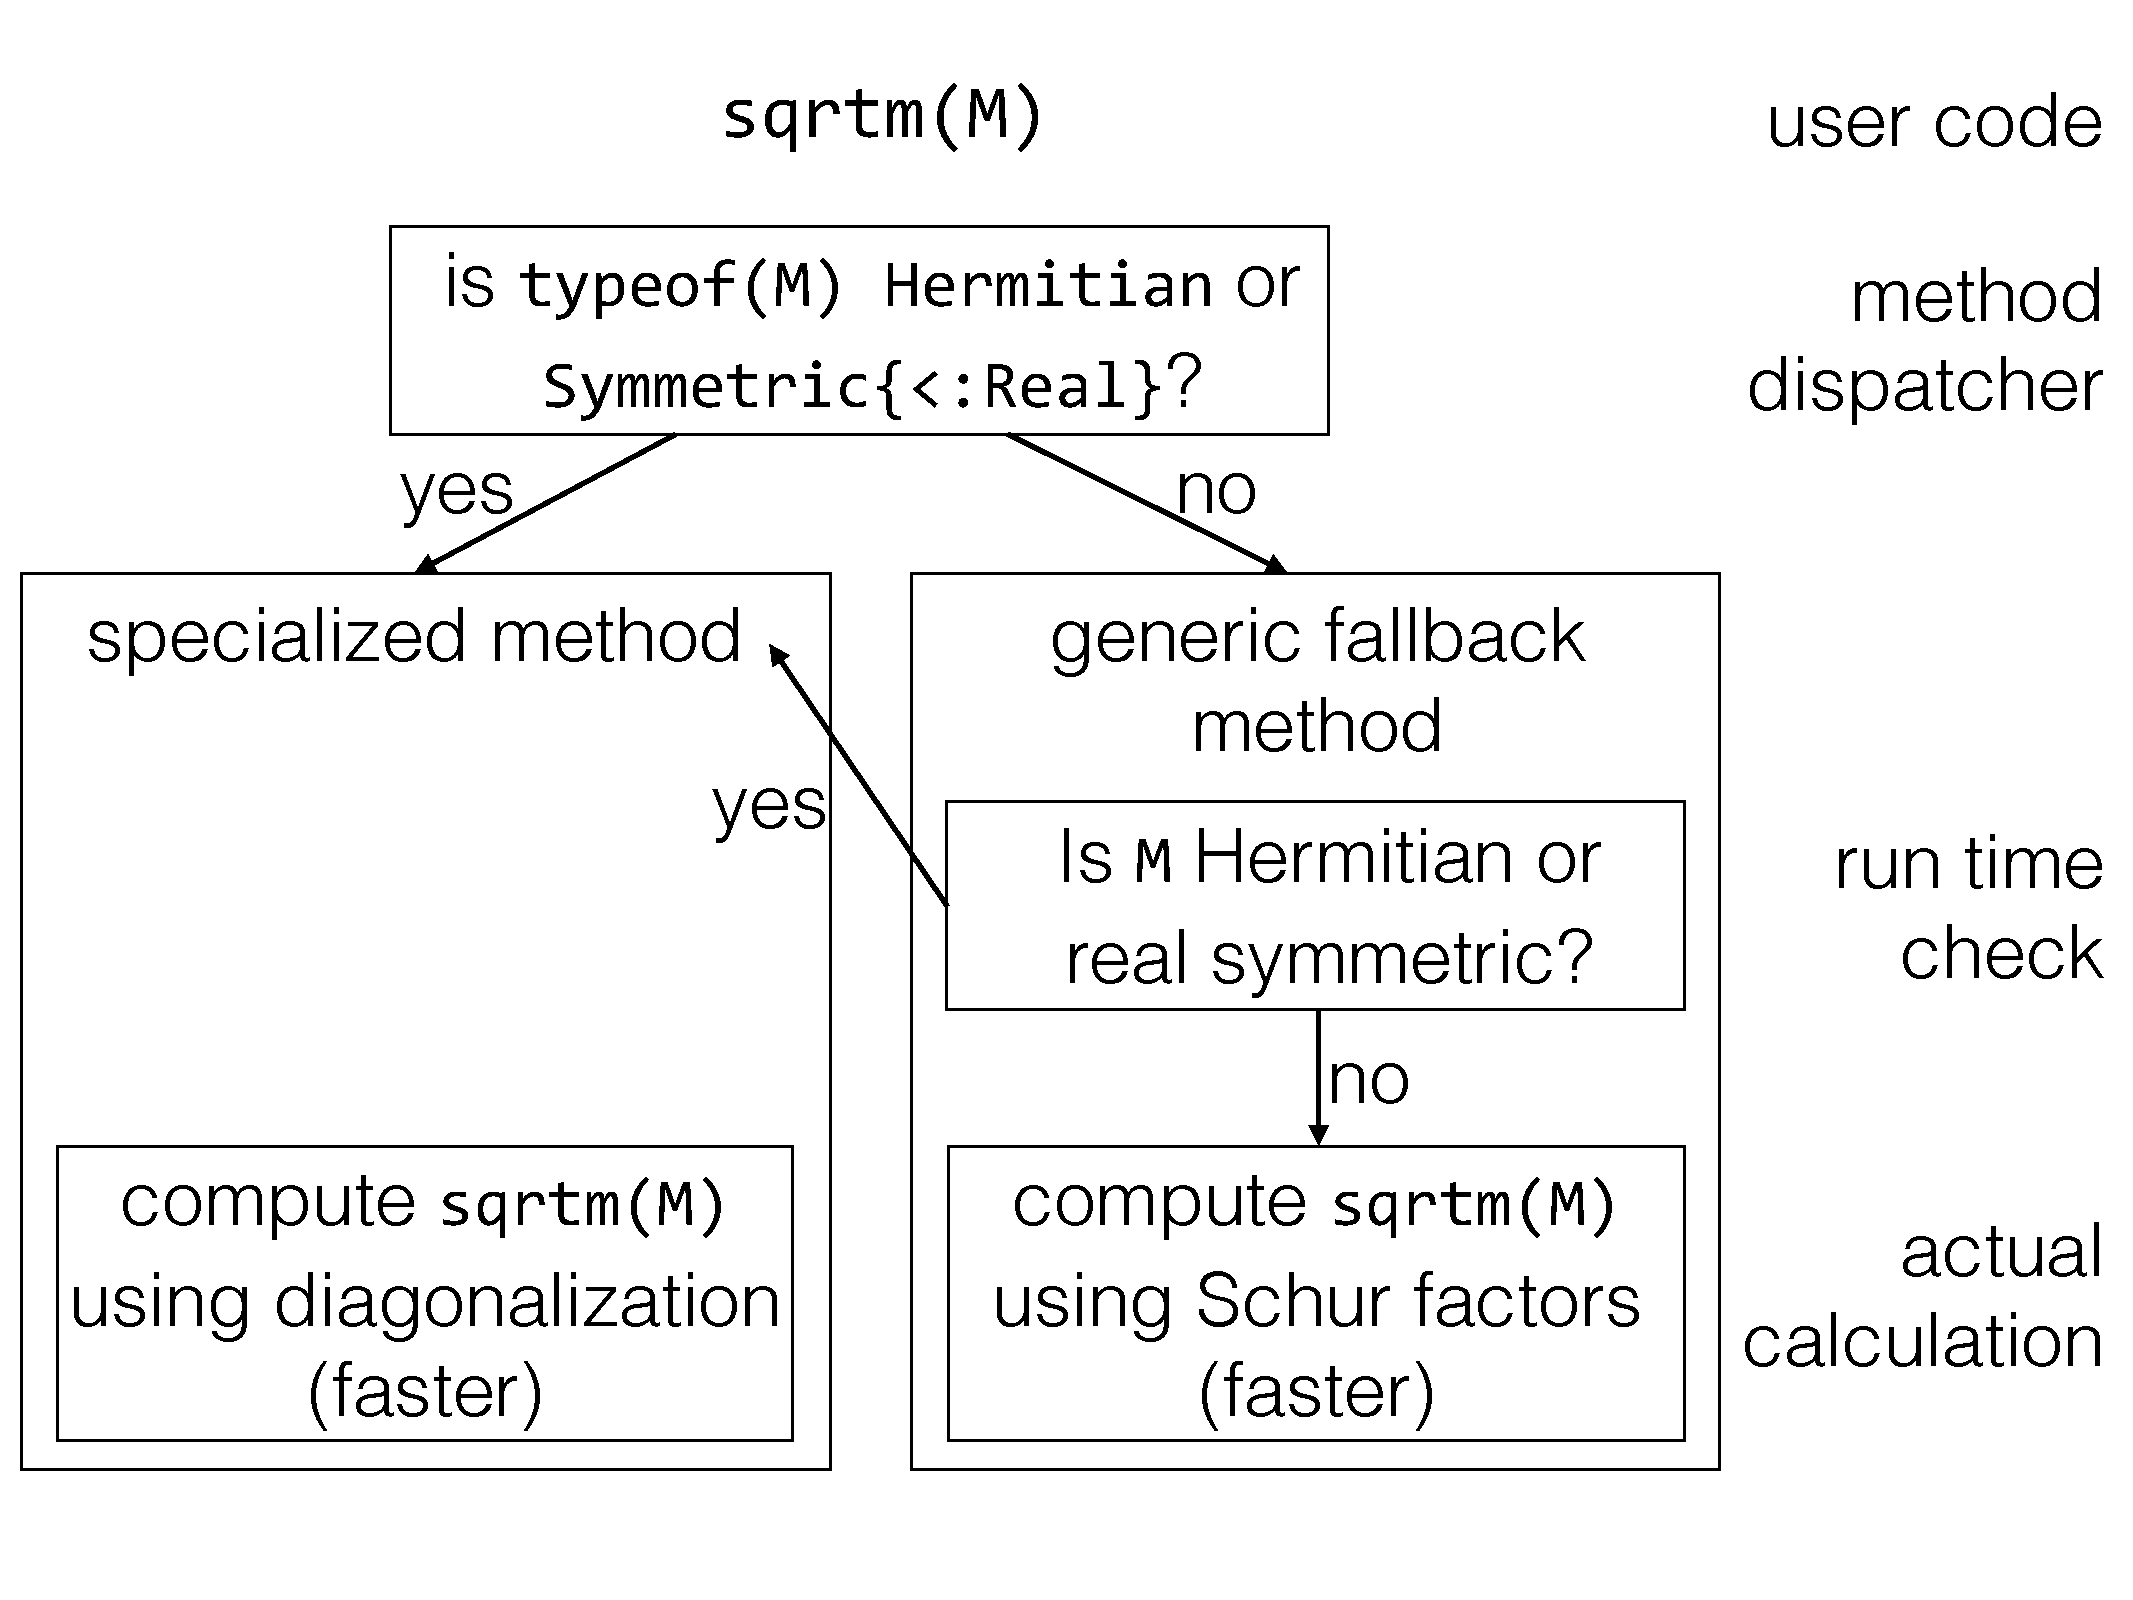
\includegraphics[width=\columnwidth]{fig-sqrtm}
	\caption{Dynamic dispatch and multimethods for the matrix square root
	function sqrtm, showing that the specialized algorithm can be
	run either from a static decision from the method dispatcher based on
	the input type, or a dynamic decision from a run time check based on
	the value.}
	\label{fig:sqrtm}
\end{figure}


\subsection{Application: statistical library routines}

\paragraph{User interpretation of generic functions}
Generic functions express a common action or computation, which may in
practice be performed in many different ways depending on the inputs. For
example, one may wish to compute the mean of a given statistical distribution.
In Julia, the computation can be expressed simply as dispatch onto the method
\code{mean(D::Distribution)}, with a different method for \code{mean} being
defined for different \code{Distribution}s. In contrast, much scientific code
is written in languages that lack generic functions, resulting in users having
to keep track of a large family of very closely related functions which
together can be thought of as specialized mthods for a polymorphic function.
Table~\ref{statsfunctions} shows a family of closely related functions in the R
programming language and their Julia counterparts in the
\package{Distributions.jl} package. Julia provides a common functional interface
for each type of statistical distribution, with generic functions like
\code{pdf} to compute the probability density function, \code{cdf} for the
cumulative density function, \code{quantile} to compute quantiles, and
\code{rand} for sampling random variates. In contrast, each distribution in R
must have its own associated family of functions prefixed by \code{d},
\code{p}, \code{q} and \code{r} respectively, and the number of functions grows
by both the number of distributions and the number of desired computations on
them.

\code{pdf}
\begin{table}
{\tiny
\begin{tabular}{l || l | l | l | l}
  \textbf{\code{D}}                & \textbf{\code{pdf(D)}}    & \textbf{\code{cdf(D)}}    &
        \textbf{\code{quantile(D)}} & \textbf{\code{rand(D)}}  \\ \hline\hline
  \textbf{\code{Beta}}             & \code{dbeta}     & \code{pbeta}     & \code{qbeta}       & \code{rbeta}    \\
  \textbf{\code{Binomial}}         & \code{dbinom}    & \code{pbinom}    & \code{qbinom}      & \code{rbinom}   \\
  \textbf{\code{Cauchy}}           & \code{dcauchy}   & \code{pcauchy}   & \code{qcauchy}     & \code{rcauchy}  \\
  \textbf{\code{Chisq}}            & \code{dchisq}    & \code{pchisq}    & \code{qchisq}      & \code{rchisq}   \\
  \textbf{\code{Exponential}}      & \code{dexp}      & \code{pexp}      & \code{qexp}        & \code{rexp}     \\
  \textbf{\code{Fdist}}            & \code{df}        & \code{pf}        & \code{qf}          & \code{rf}       \\
  \textbf{\code{Gamma}}            & \code{dgamma}    & \code{pgamma}    & \code{qgamma}      & \code{rgamma}   \\
  \textbf{\code{Geometric}}        & \code{dgeom}     & \code{pgeom}     & \code{qgeom}       & \code{rgeom}    \\
  \textbf{\code{Hypergeometric}}   & \code{dhyper}    & \code{phyper}    & \code{qhyper}      & \code{rhyper}   \\
  \textbf{\code{LogNormal}}        & \code{dlnorm}    & \code{plnorm}    & \code{qlnorm}      & \code{rlnorm}   \\
  \textbf{\code{Multinomial}}      & \code{dmultinom} & \code{pmultinom} & \code{qmultinom}   & \code{rmultinom}\\
  \textbf{\code{NegativeBinomial}} & \code{dnbinom}   & \code{pnbinom}   & \code{qnbinom}     & \code{rnbinom}  \\
  \textbf{\code{Normal}}           & \code{dnorm}     & \code{pnorm}     & \code{qnorm}       & \code{rnorm}    \\
  \textbf{\code{Poisson}}          & \code{dpois}     & \code{ppois}     & \code{qpois}       & \code{rpois}    \\
  \textbf{\code{TDist}}            & \code{dt}        & \code{pt}        & \code{qt}          & \code{rt}       \\
  \textbf{\code{Uniform}}          & \code{dunif}     & \code{punif}     & \code{qunif}       & \code{runif}    \\
  \textbf{\code{Weibull}}          & \code{dweibull}  & \code{pweibull}  & \code{qweibull}    & \code{rweibull} \\
\end{tabular}
}
\label{statsfunctions}
\caption{List of common distributions in R v3.1.1\cite{rlang} and their
associated functions. Shown in bold are the equivalent Julia generic
functions and \code{Distribution} types provided by the Julia package
\package{Distributions.jl}, showing how the namespace
is simplified by generic functions and multiple dispatch.}
\end{table}

\TODO{show code examples}

\TODO{Other possible examples from Distributions.jl: QQ plots, posterior function}

\subsection{External dispatch with dynamic multimethods}

\paragraph{writemime example}
One thing you can do with dynamic multiple dispatch is external dispatch,
i.e.\ to be able to add new methods to an existing type rather than
specifying all the possible methods upfront. This is used to good effect
in Julia packages to extend functionality of the base library. For example,
the package \package{Color.jl} for manipulating color spaces extends the
\code{writemime} base function, which writes an object as a specified
MIME type\cite{mimerfc} to an I/O stream. \code{Color.jl} extends
\code{writemime} with new methods that draw color swatches.

\TODO{Here, we could put a figure showing writemime being called on a base
Julia object, writemime(::Color), and writemime(::VectorColor) objects.
Possibly take a screenshot in IJulia.}

\paragraph{External dispatch for package interaction}
External dispatch also facilitates interaction between Julia packages---
colors can be rendered using the \package{Cairo.jl} package,
which allows rendering to a Cairo backend~\cite{cairographics}.
When using Cairo to render an object in a given color, \code{Cairo.jl}
doesn't need to know anything about the underlying color space; it just
needs to call \code{convert} methods provided by \code{Color.jl}.
Julia's \code{convert} protocol is the ``narrow waist'' that allows
packages to allow using all kinds of color spaces naturally, without
needing to know anything specifically about them.

\paragraph{External dispatch is clunky in C++}
External dispatch can be performed in other languages like C++. However,
C++ only allows static external dispatch, which severely limits its utility.
Furthermore, external dispatch in C++ requires virtual methods and visitor
patterns\cite{designpatterns} to work around the absence of explicit support
for external dispatch.



\section{Performance}


\section{Related Work}

Dynamic dispatch is more general than static dispatch since it covers cases
which cannot be determined at compile time.  Common examples involve data
retrieval with a persistent storage, generating string representations for text
output or data serialization.\cite{Shields1998}

\paragraph{Exotypes in Lua}
Exotypes\cite{exotypes} provide to the Lua language\cite{lua} the analogue of
macros that generate staged functions\cite{stagedfunc} in Julia.

There are some notable differences, though:

Exotypes are programmed in Terra,\cite{terra} a separate layer on top of the
Lua host language, and method specialization must be explicitly invoked from
within Terra. The syntax incurred by having two language layers creates an
artificial distinction between built-in methods and user-defined methods that
doesn't exist in Julia.

Exotypes implement automatic broadcasting when there is a
\code{\_\_methodmissing} property defined. Julia does not use automatic
broadcasting to implement the Proxy design pattern.

Julia uses an eager approach to resolving circularity in method definitions.
Exotypes use lazy evaluation, although interestingly, earlier versions of Terra
also used eager evaluation~\cite{terra}.

\TODO{Multiple dispatch paradigm may obviate the need for exotypes in some uses and make exotypes more powerful in others}

In a multiple dispatch paradigm, the issues brought up in Lua/Terra in wanting
to being able to create types with an unbounded number of behaviors becomes
irrelevant. There is a separation of functions and objects in Julia that
obviates the need for lazily queried properties (although it may still be a
more efficient implementation choice).

\paragraph{Dylan}

Like Julia, dispatch is dynamic, except where the compiler has determined
(possibly with sealing optimizations) that it can be optimized into a static
dispatch.

Dylan is object-oriented in the style of Common Lisp, but unlike Common Lisp,
also integrated the object system into the language.

Dylan supports a limited form of parametric types, which are called limited
types.\cite{dylanman} This allows for some modicum of generic programming.

Dylan allows structural inheritance from concrete types by structural
inheritance, i.e.\ by adding fields on top of those in the parent type. In
Julia all concrete types are final: inheritance is only allowed from abstract
types which are essentially what OO researchers call traits. Dylan lacks
traits, which are a useful mechanism for expressing generic programs.

Julia's focus is not on objects, but rather on generic and functional
programming.

Dylan supports multiple inheritance, while Julia does not and instead resorts
to duck typing.

An extension for Dylan allows for gradual typing, allowing for type information
to be determined at compile time~\cite{Mehnert2010}.

\paragraph{Dynamically-typed $\lambda$-calculus}

Several extensions of typed $\lambda$-calculus have been developed to handle
dynamic types.

One flavor is described in \cite{Henglein1994}, where a special type tag
\code{Dyn} was introduced as a placeholder type that is dynamically coerced
into other types. %But this is not the kind of polymorphism that Julia has

Other examples of coercive polymorphic $\lambda$-calculi: the $F^\uparrow_C$
language of \cite{Vytiniotis2012,haskellkindtypes} used to describe the type
inference algorithm in GHC \cite{Weirich2011} contains type coercion
information that allows type errors to deferred to runtime
\cite{Vytiniotis2012} while preserving type-correctness. (This requires
so-called kind polymorphism, which allows for programs to reason about kinds.
\cite{haskellkindtypes})

%Attempt to explain Julia's polymorphism features

However, this describes coercive polymorphism \cite{Cardelli1985}, which
is arguably not true polymorphism in the sense that it is not
universal~\cite{Strachey1967,Strachey2000}. In contrast, Julia supports two
distinct mechanisms for universal polymorphism, namely subtyping (a special
case of inclusion polymorphism), and parametric polymorphism.

Julia is not a true polymorphic system in the sense of \cite{Cardelli1985},
where code is generated only once for every generic procedure. Julia generates
a variety of specialized methods and so are more in the send of Ada-style
generic procedures which are abbreviations for sets of monomorphic procedures.

%Staged functions, dynamic λ-calculus, gradual typing... all seem to be closely related aspects of the same thing: it is often advantageous to split the determination of type information between compile time and runtime.

\paragraph{Haskell}

The main strategy in Haskell to deal with types that are not statically
decidable is to use staged type inference.~\cite{Shields1998}

\TODO{
Dynamic typing in polymorphic languages
M. Abadi, L. Cardelli, B. Pierce and D. Rémy Journal of Functional Programming / Volume 5 / Issue 01 / January 1995, pp 111 - 130 DOI: 10.1017/S095679680000126X
}

\section{Conclusions}

\paragraph{Logical challenges of parametric invariance}
Invariance is useful for things like arrays but they can make mathematical
reasoning tricky when the parametric type is something like complex.  Subtyping
is not embedding.

\paragraph{Nonobvious consequences}

A nonobvious consequence of the invariance of type parameters is that
parametric types can be instantiated with any type parameter regardless of
whether it is abstract or concrete.

The three \code{Complex} numbers

\begin{minted}{julia}
z1 = Complex{Float64}(0.0, 1.0)
z2 = Complex{FloatingPoint}(0.0, 1.0)
z3 = Complex{Union(Rational, Integer, Float64)}(0, 1.0)
\end{minted}

are all numerically equivalent (i.e.\ \code{z1 == z2 == z3}), but they are not
identical (in the \textit{egal} sense).

If we inspect the variables using Julia's \code{dump} command, we get:

\begin{minted}{jlcon}
julia> dump(z1)
Complex{Float64} 
  re: Float64 0.0
  im: Float64 1.0

julia> dump(z2)
Complex{FloatingPoint} 
  re: Float64 0.0
  im: Float64 1.0

julia> dump(z3)
Complex{Union(Integer,Float64,Rational{T<:Integer})} 
  re: Int64 0
  im: Float64 1.0

\end{minted}

We see that the \code{::T} annotation on a field does not guarantee that the
type of a value placed in the field in any given instance of that type is
exactly of type \code{T}, merely that it is a subtype of \code{T}.


\paragraph{Parametric invariance interacts with dataflow in nonobvious ways}
Parametric invariance makes it easy to construct monotone flow functions
because the underlying type lattice lends naturally to disentangled finite
chains and there is a lot more disjoint functions.
Parametric invariance makes it easy to construct monotone flow functions
because the underlying type lattice lends naturally to disentangled finite
chains and there is a lot more disjointedness to the lattice.


The 1,2,Nat example and the induced structures on \verb|S{#} <: T{#}| make for
interesting flow functions.

Consider the flow function \verb|# -> S{#}|.

It is not distributive.
flow functions need not be distributive. Distribution is desirable because it
guarantees that merging information before function application does not result
in loss of precision. However the presence of types with invariant parameters
leads naturally to consider flow functions that are NOT distributive.

\paragraph{Recursive functions are problematic to infer}

\paragraph{Widening heuristics are challenging to design}
It is not obvious how to choose widening heuristics. Widening is NOT
commutative with arbitrary flow function. This example is a direct
counterexample to the intuition that widening (pessimizing) after analysis
produces the same result as analyzing after pessimizing. In fact, in this case
we cannot say that one has a subtype relation to the other, so that in general
switching the order of flow function application and widening can produce
different results which are neither tighter nor narrower approximations, but
merely different in general.

\paragraph{Type inference on infinite lattice}
Hard to do type inference on infinite lattice. We have infinities because of
typevars and infinite tuples.  In practice there are heuristics built into type
inference which trigger widening (pessimizing), such as maximum lengths of
unions and tuples, and the maximal depths of types and tuples analyzed.
 

\paragraph{Many unexplored implementation challenges}
Possibly peephole optimizations. Constant propagation. Backward type inference.
More convoluted thingies with a general abstract interpretation framework.



\acks{We thank the many Julia users and developers for their contributions to
the Julia language.}

\listoftodos %TODO remove from final submission

\bibliographystyle{abbrvnat}
\bibliography{pldi2015,websites}

\end{document}
